\documentclass[a0paper,portrait]{baposter}

\usepackage{wrapfig}
\usepackage{lmodern}

\usepackage[utf8]{inputenc} %unicode support
\usepackage[T1]{fontenc}

\selectcolormodel{cmyk}
\graphicspath{{figures/}} % Directory in which figures are stored

\newcommand{\compresslist}{%
\setlength{\itemsep}{0pt}%
\setlength{\parskip}{1pt}%
\setlength{\parsep}{0pt}}

\newcommand{\heading}[1]{\textbf{\color{darkgreen}#1}} % highlight text with darkgreen color

\newenvironment{boenumerate}
{\begin{enumerate}\renewcommand\labelenumi{\textbf\theenumi.}}
{\end{enumerate}}

\begin{document}
\definecolor{darkgreen}{cmyk}{0.8,0,0.8,0.45}
\definecolor{lightgreen}{cmyk}{0.8,0,0.8,0.25}

\begin{poster}{
		grid=false,
		columns=2, %number of columns
		headerborder=open, % Adds a border around the header of content boxes
		colspacing=1em, % Column spacing
		bgColorOne=white, % Background color for the gradient on the left side of the poster
		bgColorTwo=white, % Background color for the gradient on the right side of the poster
		borderColor=darkgreen, % Border color
		headerColorOne=lightgreen, % Background color for the header in the content boxes (left side)
		headerColorTwo=lightgreen, % Background color for the header in the content boxes (right side)
		headerFontColor=white, % Text color for the header text in the content boxes
		boxColorOne=white, % Background color of the content boxes
		textborder=rounded, %rectangle, % Format of the border around content boxes, can be: none, bars, coils, triangles, rectangle, rounded, roundedsmall, roundedright or faded
		eyecatcher=false, % Set to false for ignoring the left logo in the title and move the title left
		headerheight=0.11\textheight, % Height of the header
		headershape=rounded, % Specify the rounded corner in the content box headers, can be: rectangle, small-rounded, roundedright, roundedleft or rounded
		headershade=plain,
		headerfont=\Large\textsf, % Large, bold and sans serif font in the headers of content boxes
		linewidth=2pt % Width of the border lines around content boxes
	}{}
	%----------------------------------------------------------------------------------------
	%	TITLE AND AUTHOR NAME
	%----------------------------------------------------------------------------------------
	{\vspace{1em}
		\textsf %Sans Serif
		{Robotic Cloth Manipulation for Clothing Assistance Task using Dynamic Movement Primitives}
	} % Poster title
	{\sf\vspace{0.1em}\\
		Ravi Prakash Joshi (Shibata laboratory)
		\vspace{0.1em}\\
		\small{Graduate School of Life Science and Systems Engineering, Kyushu Institute of Technology, 2-4 Hibikino, Kitakyushu 808-0196, Japan}}
	{
\includegraphics[trim={5mm 5mm 30mm 10mm}, clip, width=4cm]{logo}} % University/lab logo


	\headerbox{Introduction}{name=introduction,column=0,row=0, span=2}{
		The need of Robotic Clothing Assistance in the field of assistive robotics is growing, as it is one of the most basic and essential assistance activities in the daily life of elderly and disabled people. Robotic Cloth Manipulation task deals with putting a clothing article on both the arms. %The problem of robotic clothing assistance is truly confounded as there exist various failure scenarios such as performing co-operative manipulation with the human whose posture may vary while clothing also uncertainties, in the manipulation of non-rigid and profoundly deformable clothing article. Hence the robot trajectory varies significantly for various postures of the mannequin.

		In this research, we are investigating the applicability of using Dynamic Movement Primitives (DMP) as a task parameterization model for performing clothing assistance task. We have performed experiments on soft mannequin instead of human. %An approach for estimating the hand location in 3-D space from point-cloud data is also proposed. An approach for detecting failure scenarios by making the use of end-effector forces exerted by the clothing article is also proposed. Result shows that DMPs are able to generalize movement trajectory for modified posture.
	}

	\headerbox{Experimental System}{name=setup,column=0,below=introduction,span=1}{
		\begin{wrapfigure}{l}{0.5\textwidth}
			\begin{center}
				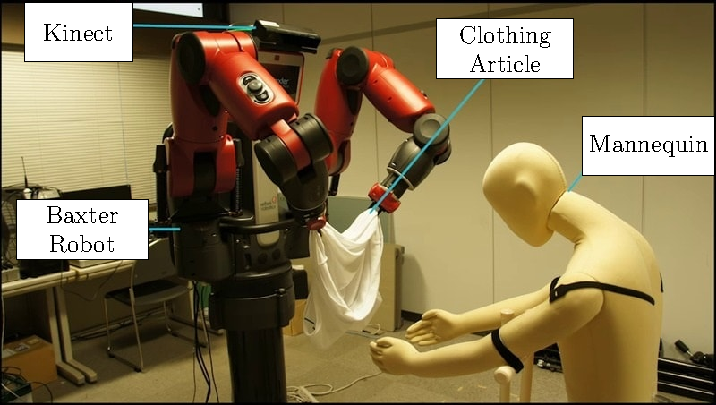
\includegraphics[width=\linewidth]{setup}
			\end{center}
		\end{wrapfigure}

		\hspace{1mm}
		\begin{center}
			\begin{itemize}\compresslist
				\item Baxter Robot
				\item Clothing Article
				\item Kinect v2
				\item Mannequin
			\end{itemize}
		\end{center}
		\vspace{10mm}
	}


	\headerbox{Experiments}{name=experiments,column=0,below=setup,span=1}{
		\begin{enumerate}\compresslist
			\item Dynamic Movement Primitives (DMP)
			\item Robotic Cloth Manipulation using DMP
			\item Estimation of Hand location in 3D space
		\end{enumerate}
	}

	\headerbox{Dynamic Movement Primitives (DMP)}{name=dmp,column=0,below=experiments,span=1}{
		Used for generating control signal to guide real system
		\begin{boenumerate}
			\item Represent policy as a non-linear dynamical system
			\item[] {\hspace{1cm} $\ddot{y} = \alpha_y ( \beta_y (g - y) - \dot{y}) + f$}
			\item[] {\hspace{1cm} $f(x,g) = \frac{\Sigma_{i=1}^N \psi_i w_i}{\Sigma_{i=1}^N \psi_i} x(g - y_0)$ where $\dot{x} = -\alpha_x x$}
			\item \textbf{Policy parameters:} Weight parameters $w_i$ used in Locally Weighted Regression
		\end{boenumerate}

		\begin{center}
			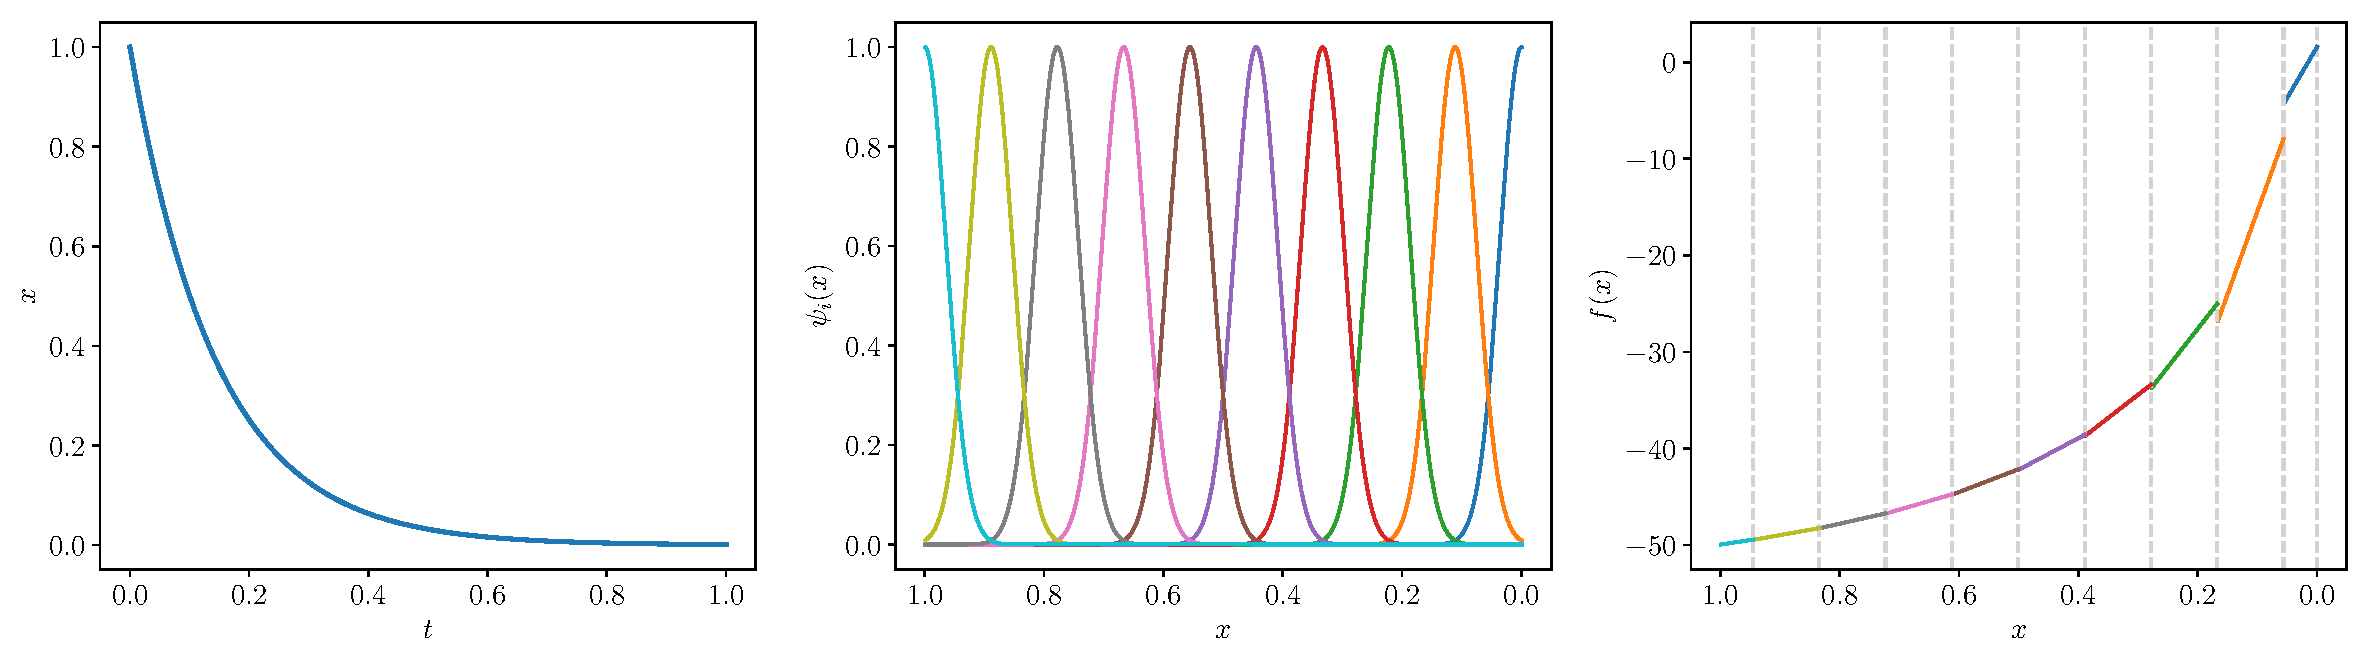
\includegraphics[trim={0 10px 0 10px}, clip, width=\textwidth]{dmp_lwr_example}
		\end{center}

		\begin{center}
			\heading{Effect of \textit{no. of basis functions}}
			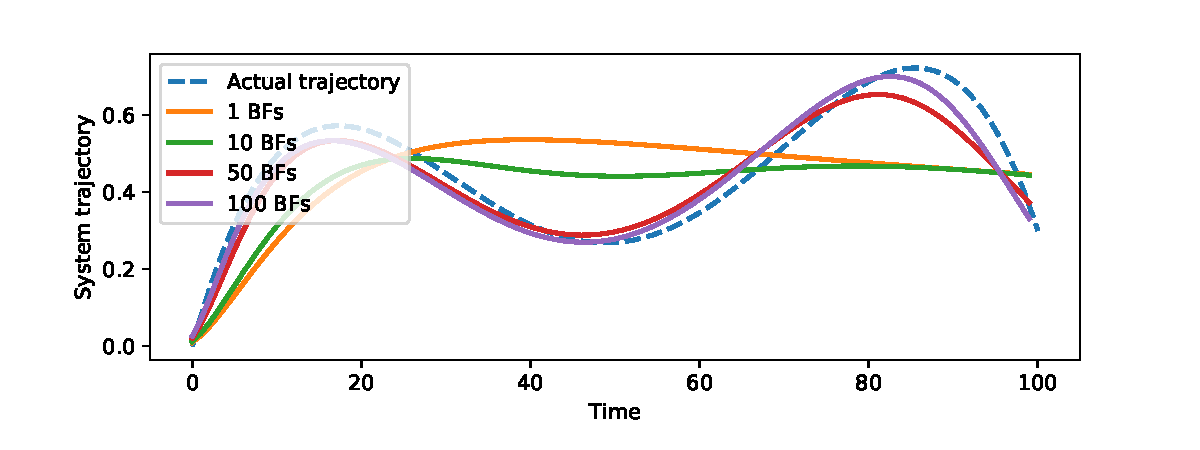
\includegraphics[trim={0 15px 0 22px}, clip, width=0.9\textwidth]{DMP_BFs}

			\heading{DMP adaptation to new goal}
			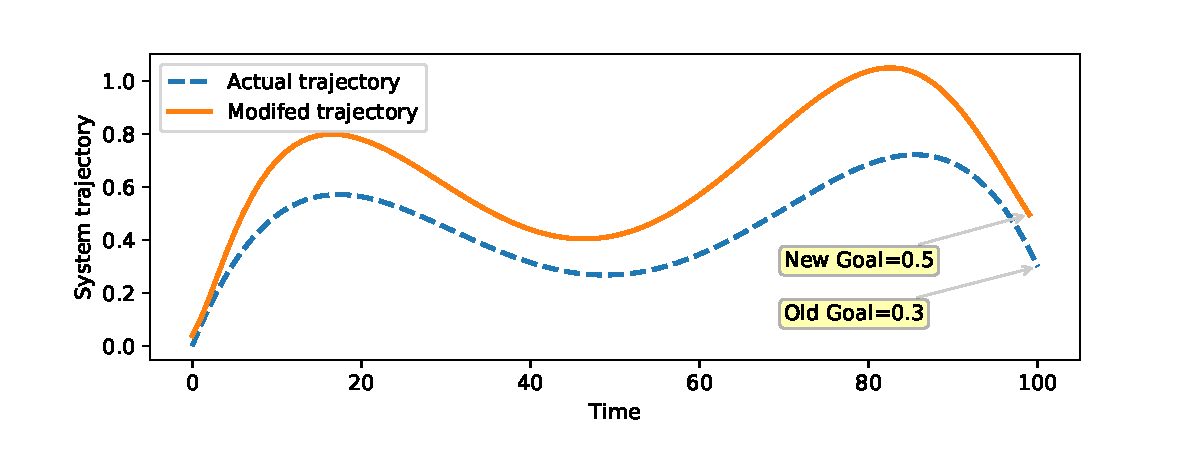
\includegraphics[trim={0 14px 0 22px}, clip, width=0.9\textwidth]{DMP_Goal}
		\end{center}
	}


	\headerbox{Robotic Cloth Manipulation using DMP}{name=rcm,column=1,below=introduction,span=1}{
		\begin{center}
			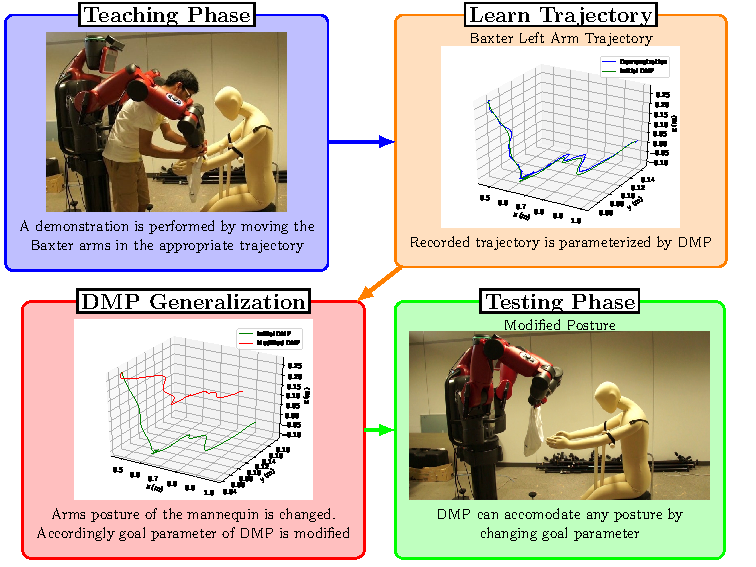
\includegraphics[width=\textwidth]{flowchart_beamer}
		\end{center}

		\begin{center}
			\heading{Accuracy measurement}
		\end{center}

		\begin{center}
			\vspace{-2mm}
			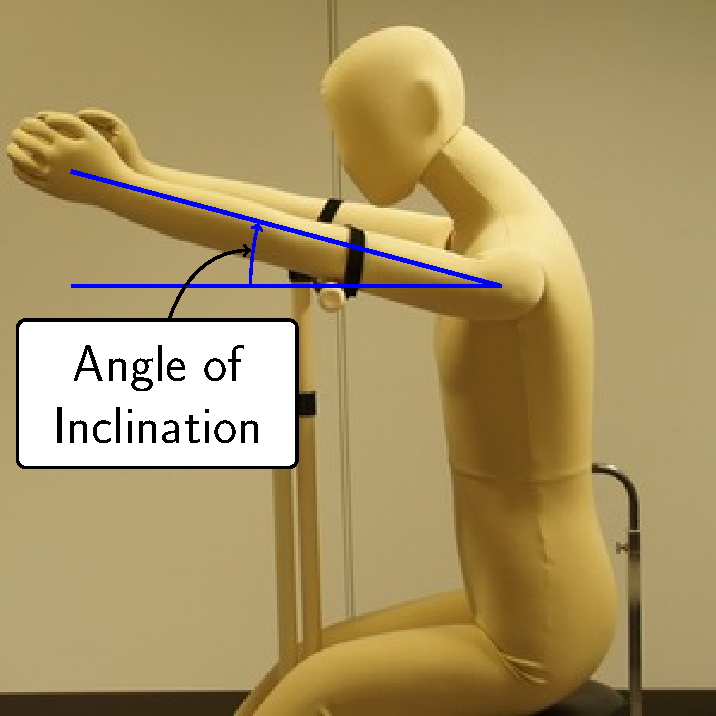
\includegraphics[width=0.44\textwidth]{inclination_plus}%continue to same line
			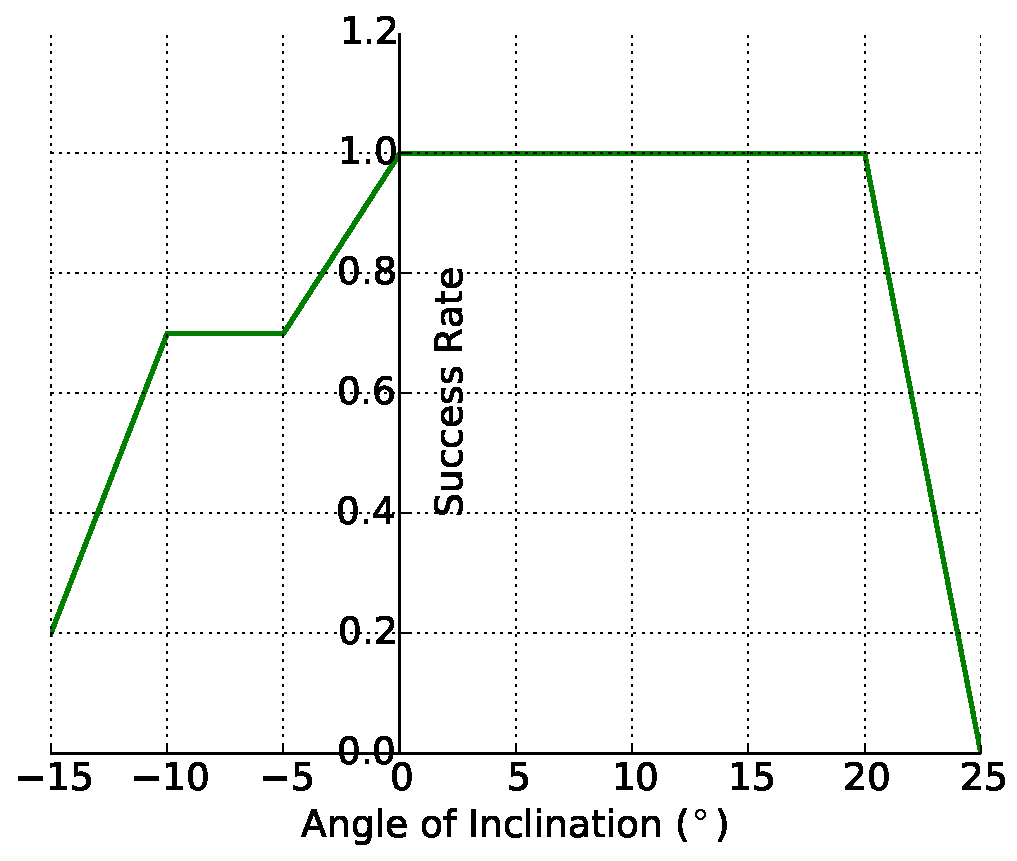
\includegraphics[width=0.55\textwidth]{success_rate}
		\end{center}
	}


	\headerbox{Estimation of Hand location in 3D space}{name=estimation,column=1,below=rcm,span=1}{
		% https://tex.stackexchange.com/a/84148
		\tikzfading[name=arrowfading, top color=transparent!0, bottom color=transparent!95]
		\tikzset{arrowfill/.style={#1,general shadow={fill=black, shadow yshift=-0.8ex, path fading=arrowfading}}}
		\tikzset{arrowstyle/.style n args={3}{draw=#2,arrowfill={#3}, single arrow,minimum height=#1, minimum width=2cm, single arrow,
			single arrow head extend=.3cm,}}

		% https://tex.stackexchange.com/a/376283
		\begin{center}
			\begin{tikzpicture}
				\node(a){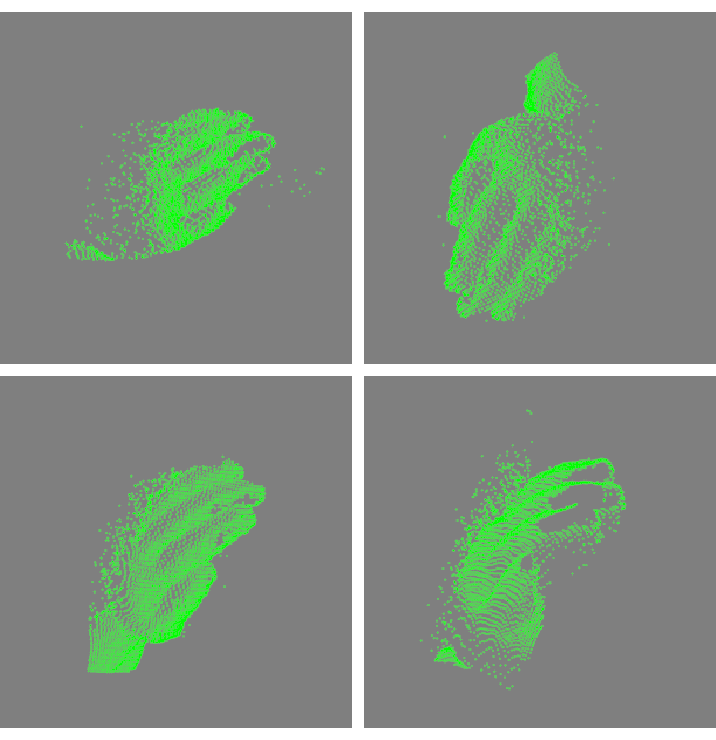
\includegraphics[width=0.3\textwidth]{wrist_images}};
				\node at (a.east)%
				[anchor=center,
					xshift=60mm,
					yshift=0mm
					]{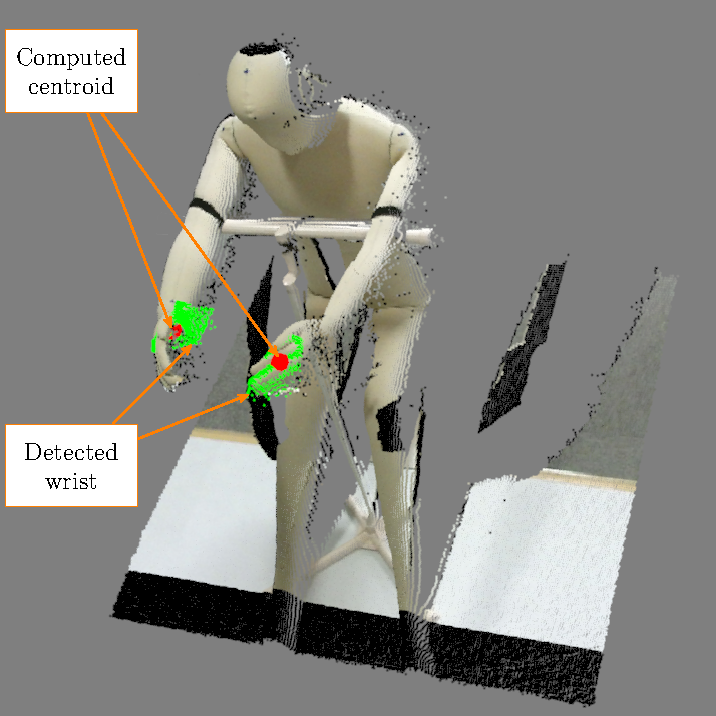
\includegraphics[width=0.3\textwidth]{wrist_detection_output}};
						\node at (a.east)[xshift=20mm, arrowstyle={3cm}{FireBrick}{top color=OrangeRed!20, bottom color=Red}] {Template Matching};
					\end{tikzpicture}
				\end{center}
			}

			\headerbox{Conclusion}{name=conclusion,column=1,below=estimation,span=1}{
				\begin{boenumerate}\compresslist
					\item Robotic clothing assistance is challenging since it requires cooperative manipulation
					\item Clothing article inherits non-rigid and highly deformable properties
					\item Real-time tracking of mannequin for making approach more robust
					\item Result shows that DMPs are able to generalize the movement trajectory
				\end{boenumerate}
			}

			\headerbox{Acknowledgments}{name=acknowledgments,column=1,below=conclusion,span=1}{
				This work was supported in part by the Grant-in-Aid for Scientific Research from Japan Society for the Promotion of Science (No. 16H01749).
			}

			\headerbox{Publications}{name=publications,column=0,below=dmp,span=1}{
				\footnotesize % Reduce the font size in this block
				\renewcommand{\section}[2]{\vskip 0.05em} % Get rid of the default "References" section title
				\nocite{*} % Insert publications even if they are not cited in the poster

				\bibliographystyle{unsrt}
				\bibliography{poster} % Use sample.bib as the bibliography file
			}
		\end{poster}
\end{document}
